\documentclass[10pt]{article}

% --- NeurIPS-style page geometry ---
\usepackage[letterpaper, top=1in, bottom=1in, left=1.2in, right=1.2in]{geometry}
\usepackage[T1]{fontenc}
\usepackage[utf8]{inputenc}
\usepackage{lmodern,microtype}
\usepackage{amsmath,amssymb,amsthm,mathtools}
\usepackage{graphicx}
\usepackage{booktabs}
\usepackage{tabularx}
\usepackage[hidelinks]{hyperref}
\usepackage{caption}
\usepackage{subcaption}
\usepackage{float}
\usepackage{enumitem}
\usepackage{titlesec}
\usepackage{multicol}
\setlength{\parskip}{1.5pt}
\setlength{\parindent}{0pt}
\titleformat{\section}{\normalsize\bfseries}{\thesection}{0.5em}{}
\titleformat{\subsection}{\small\bfseries}{\thesubsection}{0.5em}{}
\titlespacing*{\section}{0pt}{6pt}{2pt}
\titlespacing*{\subsection}{0pt}{4pt}{1pt}
\captionsetup{font=small,labelfont=bf,skip=2pt}
\captionsetup[sub]{font=small,labelfont=bf,skip=1pt}

\DeclareMathOperator*{\argmax}{arg\,max}
\DeclareMathOperator{\KL}{KL}
\newcommand{\R}{\mathbb{R}}
\newcommand{\D}{\mathcal{D}}
\newcommand{\Aspace}{\mathcal{A}}
\newcommand{\bcpol}{\pi_{\mathrm{BC}}}
\newcommand{\rb}{\bar{r}}
\newcommand{\Q}{\mathcal{Q}}
\newcommand{\V}{\mathcal{V}}

\begin{document}

\noindent\textit{\textbf{Two hypotheses are tested.}
\textbf{(H1)}~Both CSIL and CSIL+SOAR improve over BC across
$K\!\in\!\{20,50,100\}$ expert trajectories on Acrobot.
\textbf{(H2)}~SOAR provides no improvement over plain CSIL in the
discrete, reduced-budget regime considered here. Hypothesis (H2) is
stated a priori: \cite{viel2025ilsoar}~\S6 reports SOAR gains only on
continuous, higher-dimensional MuJoCo environments at $5$M env steps,
whereas the setup studied here is small, discrete, and $10\times$
below that budget.}

% ====================================================================
\section{Coherent Soft Imitation Learning (CSIL)}\label{sec:csil}
% ====================================================================

CSIL combines behavioural cloning (BC) and inverse reinforcement
learning (IRL) by using the BC policy as both a \emph{reward generator}
and a \emph{critic initialiser}. The construction relies on the
entropy-regularised soft Bellman equation
$\Q(s,a)=r(s,a)+\gamma\,\mathbb{E}_{s'}[\V_\alpha(s')]$, whose
fixed-point policy admits the Boltzmann form
$q_\alpha(a|s)\propto p(a|s)\exp(\alpha^{-1}\Q(s,a))$
(\cite{watson2023csil}~Eq.~4) for a prior $p$ and temperature $\alpha$.

\subsection{The coherent reward and its derivation}

Inverting the Boltzmann form for $\Q$ yields
$\Q(s,a)=\alpha\log\!\big(q_\alpha(a|s)/p(a|s)\big)+\V_\alpha(s)$
(Theorem~1 of~\cite{watson2023csil}). Applying the Ng--Harada--Russell
shaping lemma~\cite{ng1999shaping} with potential
$\Psi(s)\!=\!-\V_\alpha(s)$ cancels the bootstrap, leaving the
\emph{coherent reward} (Definition~1 of~\cite{watson2023csil})
\begin{equation}\label{eq:rbar}
  \rb(s,a) \;=\; \alpha\,\log\!\big(q_\alpha(a|s)/p(a|s)\big),
\end{equation}
for which $q_\alpha$ is provably soft-optimal at temperature $\alpha$.
For our discrete action spaces we set the prior to uniform,
$p(a|s)\!=\!1/|\Aspace|$, so $\log p\!=\!-\log|\Aspace|$ is a constant
and~\eqref{eq:rbar} reduces to a shifted log-likelihood of $\bcpol$.

\subsection{Three-stage training pipeline (Algorithm 1)}

\textbf{Stage~A --- BC.} $\theta_1=\argmax_\theta\,\mathbb{E}_\D[\log
q_\theta(a|s)]-\Psi(\theta)$ with weight-decay regulariser $\Psi$ and
patience-based ($P\!=\!500$) early stop on a held-out cross-entropy
split (\cite{watson2023csil}~\S{}L: ``\emph{if the policy is trained
too long, the entropy is reduced too far, and there is not enough
exploration for RL}'').

\textbf{Stage~B --- SARSA warm-up.} We initialise $Q_\phi$ via
TD-SARSA on expert transitions with the frozen reward
$\rb_{\theta_1}$ and target
$y\!=\!\rb_{\theta_1}(s,a)+\gamma(1-d)\,Q_{\bar\phi}(s',a')$, matching
$Q_\phi$ to $\bcpol$ before any environment interaction.

\textbf{Stage~C --- SAC fine-tune, $\beta\!<\!\alpha$.} The actor
maximises the KL-anchored SAC objective
$\mathcal{J}_\pi\!=\!\mathbb{E}_{a\sim q_\theta}\![Q-\beta(\log q_\theta-\log\bcpol)]$
(\cite{watson2023csil}~Eq.~5); the critic regresses to
$y=\rb_{\theta_1}+\gamma(1-d)\,\mathbb{E}_{a'\sim q_\theta}[Q_{\bar\phi}(s',a')-\beta(\log q_\theta(a'|s')-\log\bcpol(a'|s'))]$.
The strict inequality $\beta\!<\!\alpha$ (asserted at runtime in
\texttt{CSILAgent.\_\_init\_\_}) is required: at $\beta\!=\!\alpha$
the soft-optimal policy of $\rb$ is $\bcpol$ itself, so Stage~C
cannot improve on BC. Lowering $\beta$ loosens the KL anchor and
lets SAC exploit environment data.

\subsection{Algorithm 2 actor reward refinement}

Beyond $\mathcal{J}_\pi$, we use the actor-side reward refinement of
\cite{watson2023csil}~Eq.~11--12, which minimises Schulman's
positively-constrained KL estimator:
\begin{equation}\label{eq:Jr}
  -\mathcal{J}_r(\theta) \;=\; -\,\mathbb{E}_{(s,a)\sim\D}[\rb_\theta]
  + \mathbb{E}_{(s,a)\sim\rho_\pi}[\rb_\theta-1+\exp(-\rb_\theta)].
\end{equation}
A separate Adam optimiser (\texttt{lr}~$\!=\!10^{-4}$) updates $\theta$
once per env-iteration. Gradient norms are clipped to $1$ and the
replay-side reward is clamped to $[-10,+\infty)$ before $\exp(-\rb)$,
since categorical $\log\bcpol$ goes to $-\infty$ as
$\bcpol(a|s)\!\to\!0$ and produced NaN gradients in early Acrobot
runs without the clamp.

\subsection{Implementation deviations}

\textbf{(i)~Critic reward.} \cite{watson2023csil}~Algorithm~2 uses the
\emph{current} $\theta$ for $\rb_\theta$ in the critic target. A
preliminary single-seed test at $K\!=\!50$ showed this closed loop
diverging on both environments (CartPole return collapsed
$500\!\to\!137$; Acrobot $-82\!\to\!\!<\!-300$ within $30$ Stage-C
iterations): the discrete categorical actor cannot absorb the
$\exp(-\rb)$ feedback at the available training budget. The critic
therefore retains the Algorithm~1 frozen-$\theta_1$ reward, and
$J_r$ refines only the actor.
\textbf{(ii)~Reward learning rate} $10^{-4}$ instead of $10^{-3}$:
the higher rate destabilises $J_r$ when categorical log-likelihoods
span $\sim\!10$ orders of magnitude on small $|\Aspace|$.

% ====================================================================
\section{IL-SOAR --- Optimistic ensemble exploration}\label{sec:soar}
% ====================================================================

IL-SOAR~\cite{viel2025ilsoar} wraps any SAC-based imitation algorithm
by replacing the single critic with an $L$-member ensemble and
aggregating into an upper-confidence estimate. Each member $\ell$ is
itself a twin pair $(Q^{(1)}_\ell,Q^{(2)}_\ell)$ trained on the
shared backup
$y_\ell=\rb+\gamma(1-d)\min(Q^{\bar{(1)}}_\ell,Q^{\bar{(2)}}_\ell)$
(Algorithm~7 of~\cite{viel2025ilsoar}; the in-pair $\min$ is SAC's
standard anti-overestimation trick).

\subsection{Optimistic aggregation}

Aggregation uses option~2 (``Mean--Std'') of
\cite{viel2025ilsoar}~Algorithm~4. We translate from the cost form
($Q=c+\gamma\max(\bar Q-\sigma,0)$, line~6) to the reward form by
flipping the sign analogously to footnote~8's twin-critic max$\to$min
convention, so the actor sees
\begin{equation}\label{eq:Qopt}
  Q_{\mathrm{opt}}(s,a)
  \;=\;\underbrace{\tfrac{1}{L}\textstyle\sum_{\ell}\,Q_\ell(s,a)}_{\bar{Q}(s,a)}
  \;+\;\mathrm{clip}\!\Big(\sqrt{\tfrac{1}{L}\textstyle\sum_{\ell}(Q_\ell(s,a)-\bar Q(s,a))^2},\,0,\,\sigma_{\mathrm{clip}}\Big),
\end{equation}
with $Q_\ell\!=\!\min(Q^{(1)}_\ell,Q^{(2)}_\ell)$ and the biased $1/L$
variance estimator (matching \cite{viel2025ilsoar}~Algorithm~5 line~4).

\subsection{Bootstrap variant and SOAR-specific deviations}

\cite{viel2025ilsoar}~Corollary~4.11 lower-bounds $L$ for
high-probability optimism, and the \S6.1 ablation (Fig.~4) confirms
that $L\!=\!1$ fails because the members collapse to identical
estimates. To keep the members independent we sample a fresh
minibatch per ensemble member at every critic step. In a diagnostic
run, a shared minibatch gave $\mathrm{std}_\ell Q \approx 0.07$ and
per-member resampling gave $\approx 0.40$, a $5.7\times$ jump;
without per-member resampling the UCB bonus is negligible.

\textbf{Two additional SOAR-specific deviations.}
(iii)~\cite{viel2025ilsoar}~Algorithm~6 (App.~F) uses $L$
\emph{independent} replay buffers with $L$ parallel rollouts. A
single shared buffer is used here, with per-critic bootstrap sampling,
since $L\!=\!4$ parallel rollouts exceed the available compute budget.
(iv)~The SOAR ensemble critics use ReLU and no LayerNorm (default
\texttt{MLP}), while the plain-CSIL critic uses ELU with LayerNorm
(\cite{watson2023csil}~\S{}L). We did not propagate the architecture
to the ensemble; this is a confound for the SOAR-vs-CSIL comparison
and we return to it in the Limitations.

\textbf{Discrete adaptations.} The uniform prior makes $\rb$ reduce to
$\alpha\log\bcpol\!+\!\mathrm{cst}$. For minimum-time tasks
($r\!\equiv\!-1$, Acrobot), \cite{watson2023csil}~\S5.3 recommends
subtracting $\sup_{a'}\rb_{\theta_1}(s,a')$ so $\rb$ stays
non-positive; the action-independent shift cancels in
$\mathcal{J}_\pi$. We enable this on Acrobot only.

% ====================================================================
\section{Experiments}\label{sec:experiments}
% ====================================================================

\subsection{Setup}

\textbf{Environments.} \texttt{CartPole-v1} ($|\Aspace|\!=\!2$,
return cap $500$) and \texttt{Acrobot-v1} ($|\Aspace|\!=\!3$,
$r\!\equiv\!-1$). The expert is PPO from Stable-Baselines3,
trained $2\!\times\!10^5$ steps on CartPole and $5\!\times\!10^6$ on
Acrobot, with deterministic test-time action selection (stochastic PPO
sampling around saturated logits caps BC at $\sim\!-72$ on Acrobot).

\textbf{Conditions.} $K\!\in\!\{20,50,100\}$ expert trajectories,
spanning one decade of demonstration budget but staying in the regime
where BC plateaus well below the expert (initial sweeps at
$K\!\le\!10$ left BC at $\sim\!-77$, with no headroom for Stage~C).
Three seeds per cell, both algorithms on Acrobot, $18$ runs total. Stage~A: $5000$ BC steps with early stop. Stage~B: $2000$
SARSA steps. Stage~C: $480$ iterations $\times$ $1000$ env steps
($\textbf{480k env steps}$, $\approx\!6000$ episodes), with $16$
gradient steps per iteration on each of \{actor, critic\}. This budget
is $\sim\!10\!\times$ below the $5$M reported in~\cite{watson2023csil};
the $18$~benchmark cells at the full budget would require
$\sim\!7$~days of single-GPU compute, beyond the available allocation.

\textbf{Hyperparameters.} $\alpha\!=\!1$, $\gamma\!=\!0.99$, Polyak
$\tau\!=\!5\!\times\!10^{-3}$, actor/critic lr $10^{-3}$, reward lr
$10^{-4}$, batch $256$, replay $10^5$, hidden $(256,256)$.
$\beta\!=\!0.05$ (CartPole) / $0.10$ (Acrobot): \cite{watson2023csil}
Table~3 reports $\beta\!=\!0.01$ as optimal at 5M steps, but a
single-seed sweep at the $100$k-step budget showed $\beta\!=\!0.01$
destabilises the critic (the replay--$J_r$ feedback loop diverges);
we adopt the next-larger values in \cite{watson2023csil}~Table~3.
$L\!=\!4$: \cite{viel2025ilsoar}~Fig.~4 ablation shows $L\!=\!4$
recovers most of $L\!=\!16$'s performance at $1/4$ the wall-clock cost.
$\sigma_{\mathrm{clip}}\!=\!1.0$ (Acrobot): an upper bound on the
UCB bonus in the event of large ensemble disagreement. Empirically
$\mathrm{std}_\ell Q\!<\!0.7$ throughout training, so the clip is
never active.

\textbf{Evaluation protocol.} Following \cite{watson2023csil}~Fig.~4
caption, the deterministic actor is evaluated on $20$ episodes with
fixed seeds $10000\!-\!10019$ at every $n_\mathrm{iters}/10\!=\!48$
Stage-C iterations (and at $t\!=\!0$). The primary metric is the
$25\mathrm{th}$ percentile $Q_{25}$ of those $20$ returns at the
\emph{best-snapshot} checkpoint, restored before final evaluation.
$Q_{25}$ is preferred over the mean: on $N\!=\!20$ episodes a single
high-return rollout can shift the mean, whereas $Q_{25}$ reflects
the lower quartile and is less sensitive to such outliers. Standard
deviations are reported in their sample form (ddof$=$1, $N\!=\!3$
seeds).

\subsection{Main results}

We present two complementary views. Fig.~\ref{fig:curves} plots the
per-checkpoint mean return (noisy training dynamics);
Fig.~\ref{fig:cummax} plots the per-seed cumulative maximum of
$Q_{25}$ then averaged across seeds (the monotone snapshot view
of~\cite{watson2023csil}~Fig.~4, in which each y-value is the best
$Q_{25}$ if training stopped at that episode).
Table~\ref{tab:results} gives the final snapshot $Q_{25}$ per cell.

\begin{figure}[H]
  \centering
  \begin{subfigure}{0.42\linewidth}
    \centering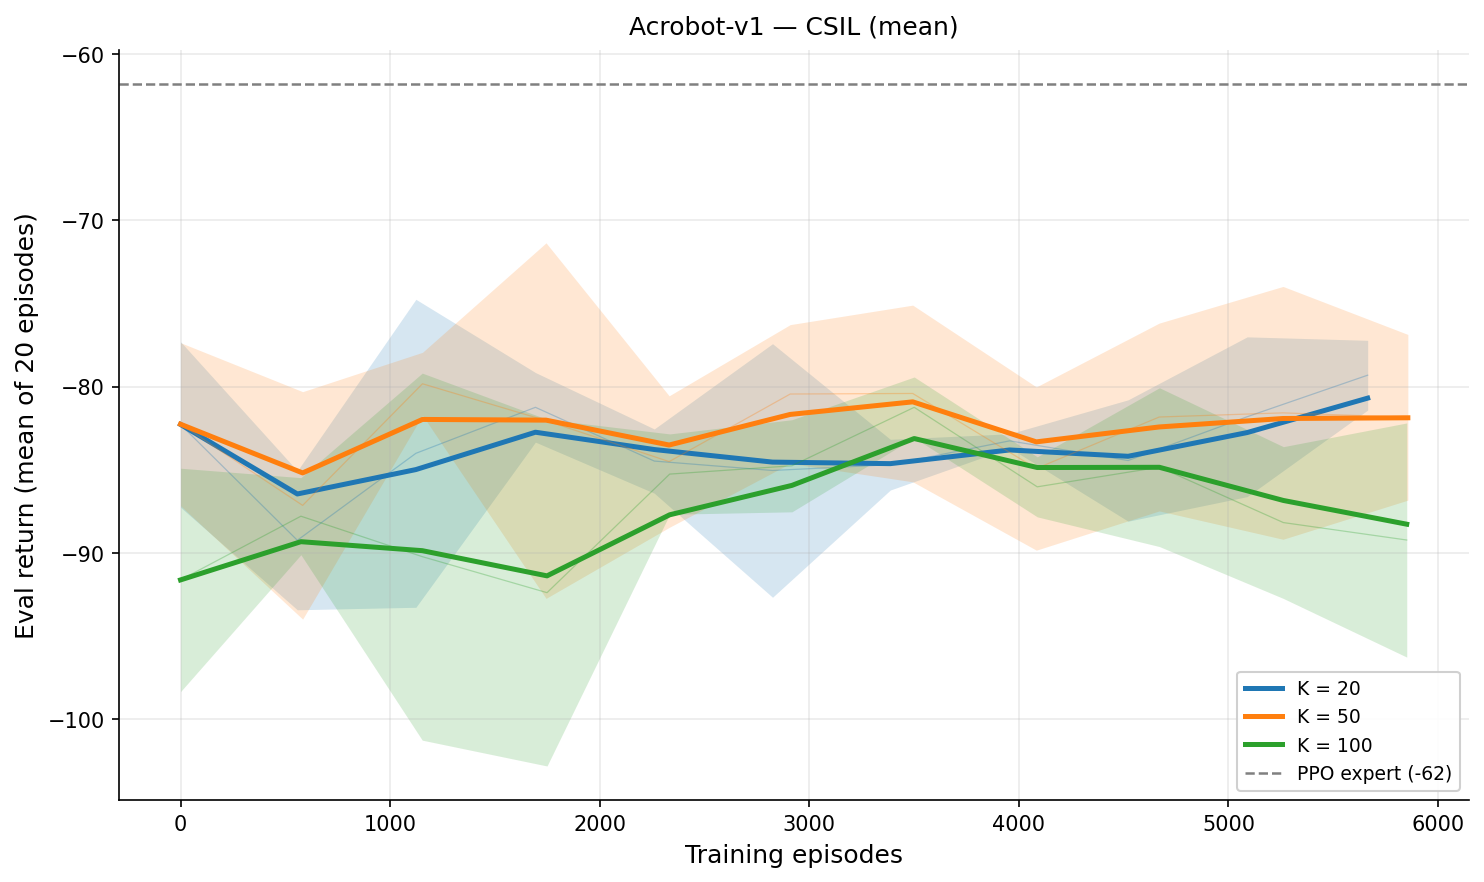
\includegraphics[width=\linewidth]{plots/acrobot_csil_mean.png}
    \caption{CSIL --- mean}\label{fig:csil_mean}
  \end{subfigure}\hspace{1em}
  \begin{subfigure}{0.42\linewidth}
    \centering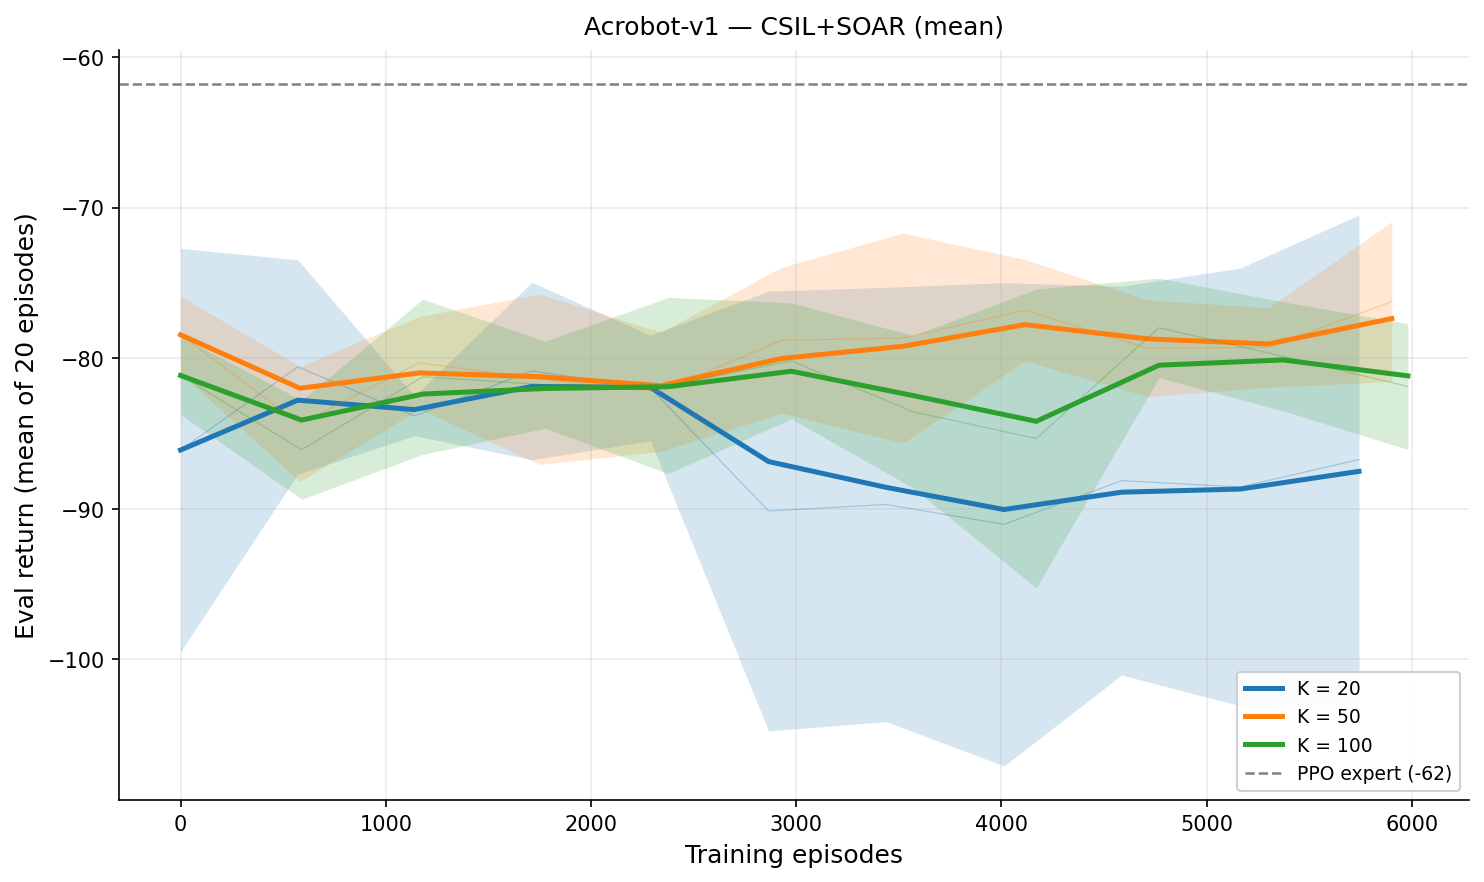
\includegraphics[width=\linewidth]{plots/acrobot_csilsoar_mean.png}
    \caption{CSIL+SOAR --- mean}\label{fig:soar_mean}
  \end{subfigure}
  \caption{\textbf{Raw training curves on Acrobot-v1, $\approx\!6000$
    Stage-C episodes.} Y: checkpoint mean return over 20
    deterministic episodes; X: cumulative training episodes;
    shaded $\pm$ one ddof$=$1 std across 3 seeds; dashed: PPO expert
    ($-61.8$). \textbf{(a)}~CSIL's gain over BC scales with $K$. \textbf{(b)}~CSIL+SOAR reaches higher plateaus at
    $K\!=\!50,100$ but visibly regresses at $K\!=\!20$ (blue): one
    seed's optimistic bonus pushed the actor away from the BC
    initialisation, dragging the mean to $\sim\!-90$ around episode
    $4000$.}
  \label{fig:curves}
\end{figure}

\begin{figure}[H]
  \centering
  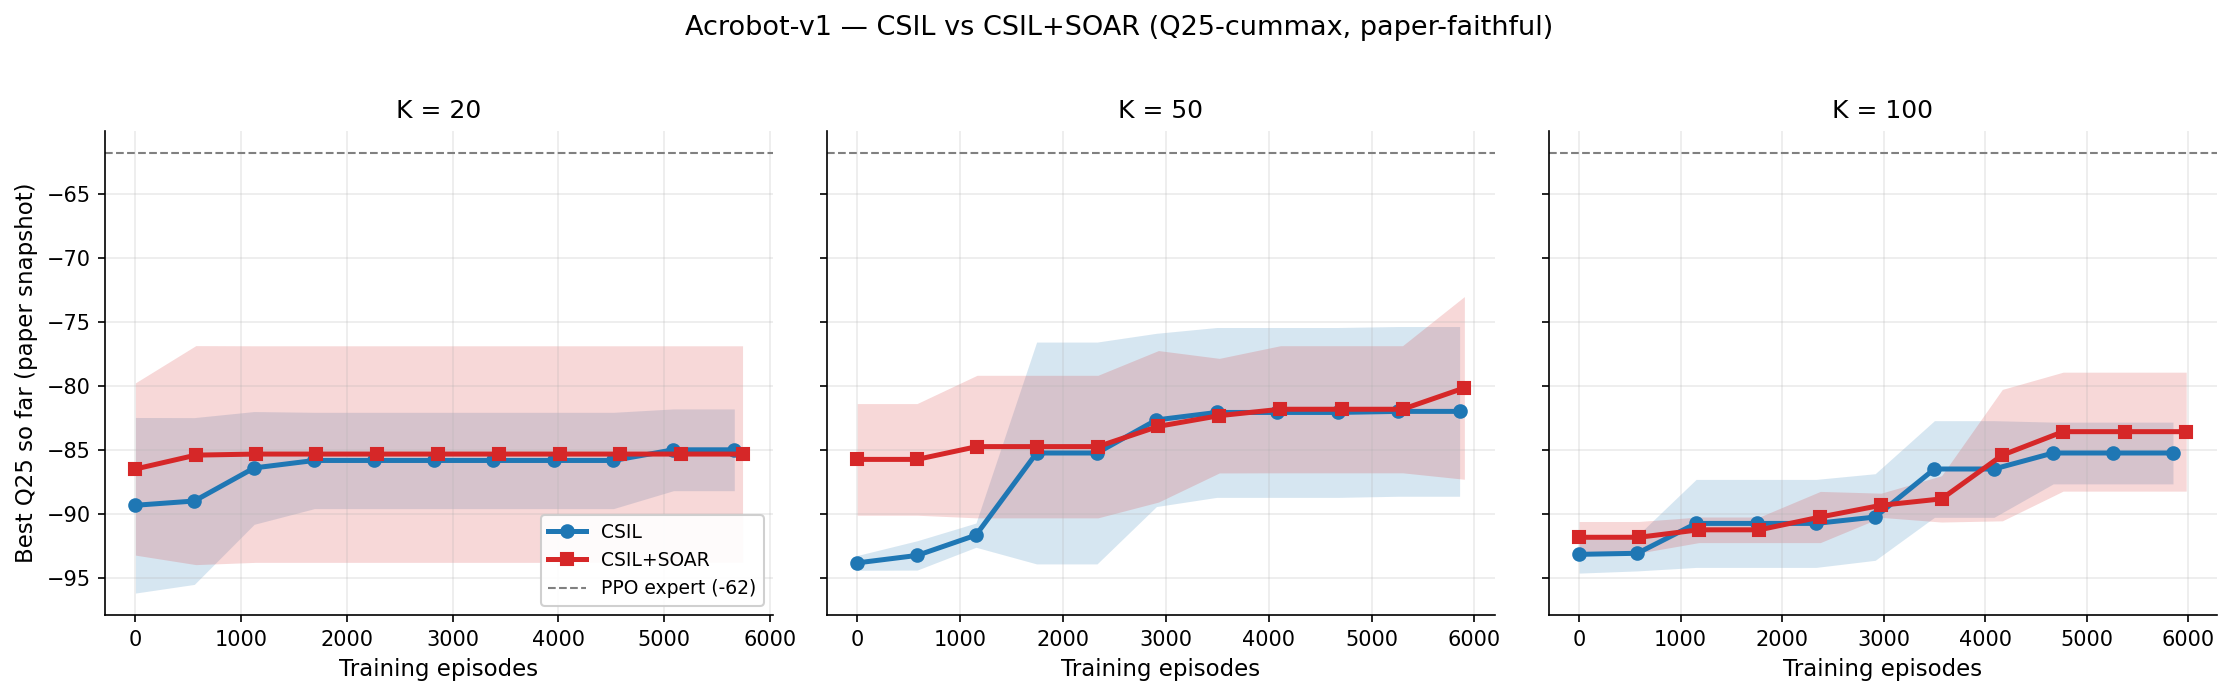
\includegraphics[width=0.66\linewidth]{plots/acrobot_compare_q25cummax.png}
  \caption{\textbf{Snapshot view: cumulative maximum of $Q_{25}$,
    CSIL vs.\ CSIL+SOAR.} Y: per-seed
    $\max_{t'\le t}Q_{25}(t')$, mean across 3 seeds; shaded
    $\pm$ ddof$=$1 std; dashed: PPO expert. Curve form of the snapshot
    protocol (\cite{watson2023csil}~Fig.~4): each y is the best
    $Q_{25}$ if training stopped at that episode. At $K\!=\!50,100$
    CSIL+SOAR (red) plateaus a few hundred episodes earlier than CSIL
    (blue) but with wider bands; at $K\!=\!20$ the two are
    statistically tied.}
  \label{fig:cummax}
\end{figure}

\begin{figure}[H]
  \centering
  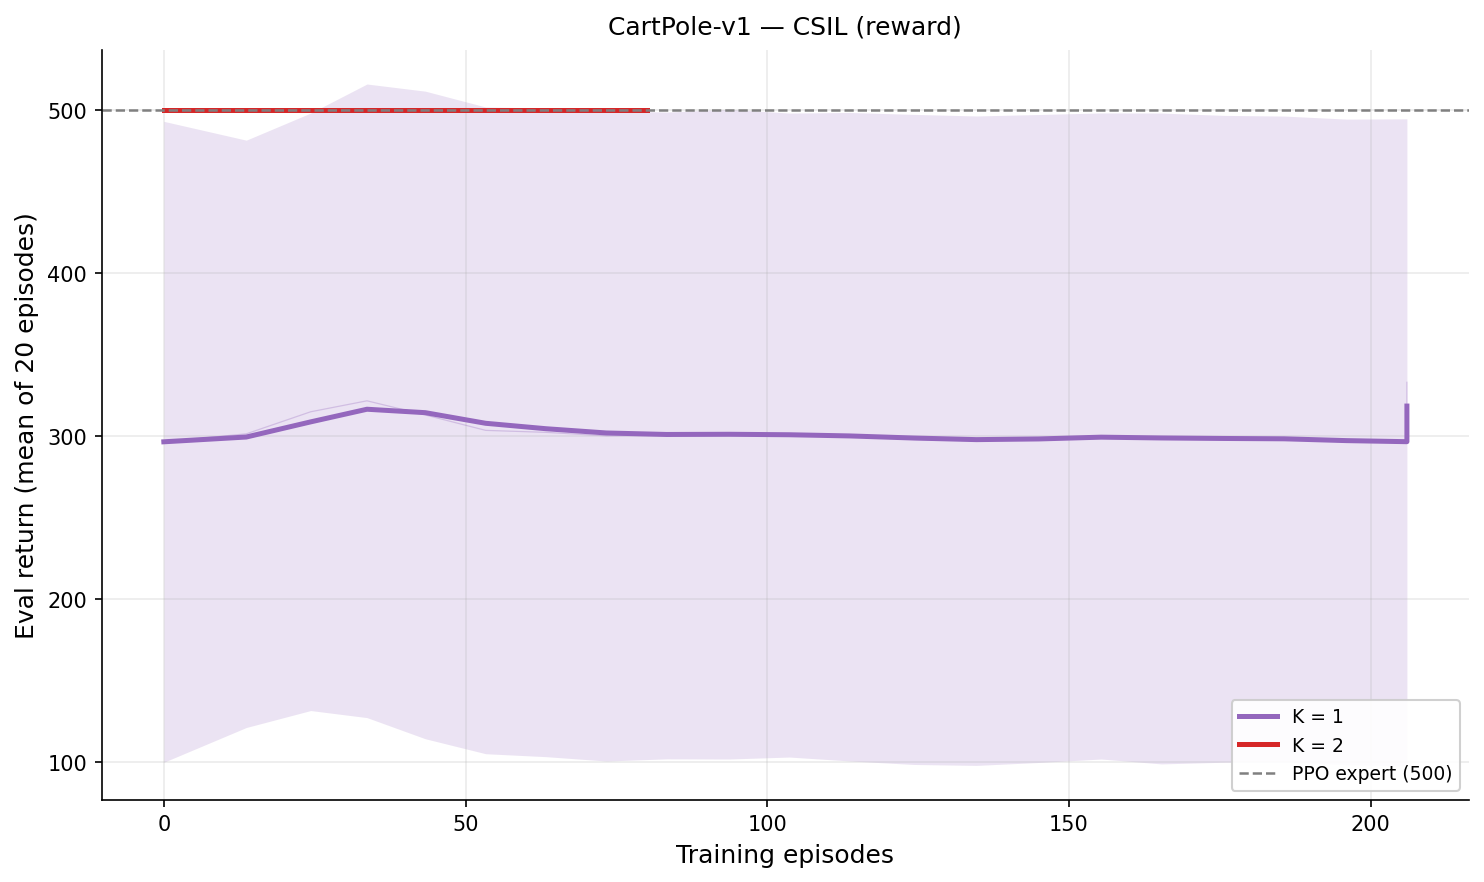
\includegraphics[width=0.38\linewidth]{plots/cartpole_csil_mean.png}
  \caption{\textbf{Why CartPole is excluded.} \texttt{CartPole-v1}'s
    state space is low-dimensional and the expert's policy is
    near-linear in the observations, so BC absorbs the expert almost
    perfectly with very little data: at $K\!=\!2$ trajectories
    ($\sim\!400$ transitions), BC already saturates the
    $500/500$ return cap (red). With $K\!=\!1$ (purple) the policy
    is still under-data and noisy. Any $K\!\ge\!20$ is therefore
    trivially capped --- Stage~C has zero headroom, and the
    CSIL-vs-SOAR contrast cannot be measured.}
  \label{fig:cartpole}
\end{figure}

\begin{table}[H]
  \centering\small
  \caption{\textbf{$Q_{25}$ at the best snapshot following
    \cite{watson2023csil}~Fig.~4, mean$\pm$ddof$=$1 std over 3 seeds.}
    The \emph{gap} is the improvement over each algorithm's own BC
    baseline (BC values differ between CSIL and SOAR runs by
    $\sim\!3$~pts because the \texttt{torch} random number generator
    advances differently in the two agent constructors; the gap is
    computed row-wise within the same random seed).
    All numbers reproduce from
    \texttt{benchmark\_csil\_Acrobot-v1.csv} and
    \texttt{benchmark\_csil\_soar\_Acrobot-v1.csv} to $\pm0.1$.
    PPO expert: $-61.8\!\pm\!0.7$.}
  \label{tab:results}
  \vspace{0.2em}
  \begin{tabular}{l c c c c c c}
    \toprule
    & \multicolumn{2}{c}{$K\!=\!20$} & \multicolumn{2}{c}{$K\!=\!50$} & \multicolumn{2}{c}{$K\!=\!100$} \\
    \cmidrule(lr){2-3}\cmidrule(lr){4-5}\cmidrule(lr){6-7}
    & $Q_{25}$ & gap & $Q_{25}$ & gap & $Q_{25}$ & gap \\
    \midrule
    BC (CSIL run)  & $-89.3\!\pm\!6.9$ & ---     & $-93.8\!\pm\!0.6$ & ---      & $-93.2\!\pm\!1.5$ & ---      \\
    CSIL           & $-85.0\!\pm\!3.2$ & $+4.3$  & $-82.0\!\pm\!6.6$ & $+11.8$  & $-85.2\!\pm\!2.4$ & $+8.0$   \\[0.2em]
    BC (SOAR run)  & $-86.5\!\pm\!6.7$ & ---     & $-85.8\!\pm\!4.4$ & ---      & $-91.8\!\pm\!1.2$ & ---      \\
    CSIL+SOAR      & $-85.3\!\pm\!8.5$ & $+1.2$  & $-80.2\!\pm\!7.1$ & $+5.6$   & $-83.6\!\pm\!4.6$ & $+8.2$   \\
    \bottomrule
  \end{tabular}
\end{table}

\subsection{Observations}

\textbf{(i)~H1 confirmed --- both CSIL and CSIL+SOAR improve BC
across all $K$.} All 6/6 (algo$\times$$K$) mean cells in
Table~\ref{tab:results} are positive; per-seed, $16/18$ gaps are
strictly positive with $2$ ties at $K\!=\!20$ and no negatives. The largest gap, $+11.8$ at
$K\!=\!50$, falls where you would expect: Stage~C has the most room
when BC covers enough state-action support to bootstrap from, but
not so much that BC already sits at the expert plateau. CSIL snapshot iterations
$t^\star\!\in\!\{0,96,144,240,288,384,432\}$: on 8/9~runs Stage~C
improves on BC for between $20\%$ and $90\%$ of the budget; on the
remaining run (seed $0$, $K\!=\!20$) Stage~C did not beat BC.

\textbf{(ii)~H2 confirmed --- CSIL+SOAR matches CSIL on the mean,
with higher variance.} SOAR is marginally better at $K\!=\!50$
($+1.8$) and $K\!=\!100$ ($+1.6$), tied at $K\!=\!20$ ($-0.3$). Across
$K$, $\bar\sigma_{\mathrm{SOAR}}\!=\!6.7$ vs.\
$\bar\sigma_{\mathrm{CSIL}}\!=\!4.1$. At $K\!=\!20$ seed~$2$, the SOAR
snapshot iteration is $t^\star\!=\!0$: \emph{every} subsequent
checkpoint had $Q_{25}\!<\!-88.5$, i.e.\ the optimistic bonus actively
prevented improvement in $1/9$ runs (visible as the blue curve in
Fig.~\ref{fig:soar_mean}). With $N\!=\!3$ seeds this comparison is
underpowered; we treat it as suggestive, not conclusive
(see~\S\ref{sec:discussion}).

\textbf{(iii)~$\sim\!20$ points remain to the expert.} Best CSIL or
SOAR $Q_{25}$ is $-80.2$ vs.\ expert $-61.8$. Our budget is
$\sim\!10\!\times$ below \cite{watson2023csil}'s $5$M; whether the
residual gap reflects insufficient interactions or an intrinsic
ceiling for our discrete actor is examined in \S\ref{sec:discussion}.

\textbf{(iv)~CartPole was excluded} (Fig.~\ref{fig:cartpole}): on this
low-dimensional task BC absorbs the expert's policy almost immediately
($K\!=\!2$ already locks in $500/500$ for both algorithms), so any
$K\!\ge\!20$ leaves Stage~C flat at the return cap with no headroom
to discriminate CSIL from CSIL+SOAR.

% ====================================================================
\section{Discussion}\label{sec:discussion}
% ====================================================================

\textbf{Why Stage~C curves stay close to BC.} The coherent reward
$\rb\!=\!\alpha\log(\bcpol/p)$ shared by CSIL and CSIL+SOAR carries
\emph{no information about the environmental goal}: its soft-optimal
policy at temperature $\alpha$ is exactly $\bcpol$ (Theorem~1).
Stage~C can only depart from BC through the $\alpha\!-\!\beta$ gap,
and $\rb$ gives no direction for that departure. The actor therefore
wanders: the raw mean (Fig.~\ref{fig:curves}) takes $+5$ to $+15$
point excursions and falls back, while the snapshot view
(Fig.~\ref{fig:cummax}, \cite{watson2023csil}~Fig.~4 protocol)
keeps the peaks. This gap between the two views explains why the
$Q_{25}$ values in Table~\ref{tab:results} record the $+4$ to $+12$
point gains of H1 even when the raw curves look flat. CSIL and CSIL+SOAR
both amplify the BC policy; neither searches for a better one.

SOAR yields no improvement over CSIL on $Q_{25}$, consistent with
\cite{viel2025ilsoar}~\S6: the ensemble bonus appears only on
continuous higher-dimensional MuJoCo environments. Our data do not separate
(\textbf{A})~SOAR is intrinsic to continuous high-dim control from
(\textbf{B})~SOAR would help here too at $5$M env steps;
discriminating would require CSIL+SOAR on Acrobot at $5$M or on
Ant-v5 at $480$k, neither done. A second regime factor compounds (B):
the discrete softmax actor with $|\Aspace|\!=\!3$ and $\beta\!=\!0.10$
is near-deterministic ($\sim\!98\%$ argmax in diagnostic runs not
re-logged), so a UCB bonus of magnitude
$\mathrm{std}_\ell Q\!\approx\!0.4$ is small next to the $\sim\!5$
$Q$-gap between actions.

\paragraph{Limitations.}
(1)~Three seeds per cell; any $\sigma$-level claim, including obs (ii),
needs $\ge\!10$ seeds before it can be taken seriously. (2)~The
$\sigma_{\mathrm{clip}}\!=\!1.0$ ceiling on Acrobot never fired in
our runs, so we have no evidence on its true sensitivity; a sweep
$\sigma_{\mathrm{clip}}\!\in\!\{0.1,0.3,0.5,1.0,2.0\}$ would settle it.
(3)~The SOAR ensemble critic uses ReLU and no LayerNorm while
plain-CSIL uses ELU and LayerNorm. Every SOAR-vs-CSIL number is
confounded by this; we would need to re-run with matched architectures
to isolate the SOAR contribution.

% ====================================================================
\vspace{2pt}{\footnotesize
\begin{thebibliography}{9}\setlength{\itemsep}{-2pt}\setlength{\parsep}{0pt}\setlength{\topsep}{-6pt}
\bibitem{watson2023csil}J.~Watson, S.~H.~Huang, N.~Heess. Coherent Soft Imitation Learning. NeurIPS 2023, arXiv:2305.16498.
\bibitem{viel2025ilsoar}S.~Viel, L.~Viano, V.~Cevher. IL-SOAR: Imitation Learning with Soft Optimistic Actor cRitic. arXiv:2502.19859, 2025.
\bibitem{haarnoja2018sac}T.~Haarnoja, A.~Zhou, P.~Abbeel, S.~Levine. Soft Actor-Critic. ICML 2018.
\bibitem{ng1999shaping}A.~Y.~Ng, D.~Harada, S.~Russell. Policy invariance under reward transformations. ICML 1999.
\bibitem{ross2011dagger}S.~Ross, G.~Gordon, J.~A.~Bagnell. A Reduction of Imitation Learning to No-Regret Online Learning. AISTATS 2011.
\end{thebibliography}}

\end{document}
